\documentclass[../main.tex]{subfiles}

\begin{document}

\section{Mesh Convergence}

The accuracy of modeling physical phenomena defined by partial differential equations depends heavily on the mesh used to discretize the problem of interest.
A mesh convergence study is crucial to maximize the confidence and efficiency of a model.
Beginning with a coarse mesh, we analyze the evolution of a specific objective function as the output changes with mesh density across increasingly resolved meshes.
\textit{Abaqus} generated a fully-quadrilateral mesh on the torque arm using the medial axis setting to create a uniform, symmetrical mesh.
The objective function tracked during the convergence study is maximum Von Mises stress for both the preload and oscillating load conditions.
The metric used to increase mesh resolution is element seed size, representative of the approximate final element size in the mesh.
Beginning with a seed size of \(5\,\unit{\milli\meter}\), six meshes were created before convergence was achieved for both load cases, using seed sizes of \(5, 4, 3, 2, 1,\,\textrm{and}\, 0.5\).
The results of the convergence study are shown in tables \ref{preload_convergence} and figure \ref{oscillating_convergence}, both of which highlight the decreasing residual change with increased element count. 
Increasing resolution beyond the 5\textsuperscript{th} mesh shows a minimal change (\(<1\%\)) in maximum Von Mises stress, indicating that the 5\textsuperscript{th} mesh is sufficiently resolved for our analysis and further refinements would only increase computational cost.
The initial, converged, and finest meshes are shown in figure \ref{meshes}.
Contour plots of Von Mises stress for the initial coarse mesh and final converged mesh, shown in figure \ref{coarse_vs_converged}, show very similar trends with the bulk qualities of the contours in agreement, though the finer details are naturally smoother and more resolved in the converged mesh.

\begin{table}[h!]
    \resizebox{\textwidth}{!}{%
    \begin{tabular}{|lllllll|}
    \hline
    \multicolumn{7}{|c|}{Preload Convergence History}                                                                                                                                                                                                                                      \\ \hline
    \multicolumn{1}{|l|}{Mesh Iteration} & \multicolumn{1}{l|}{Seed Size} & \multicolumn{1}{l|}{Number of Elements} & \multicolumn{1}{l|}{Element Type} & \multicolumn{1}{l|}{Element Size (Critical Region)} & \multicolumn{1}{l|}{Von Mises Stress (MPa)} & \% Change from Previous Mesh \\ \hline
    \multicolumn{1}{|l|}{1}              & \multicolumn{1}{l|}{5}         & \multicolumn{1}{l|}{204}                & \multicolumn{1}{l|}{CPS8R}        & \multicolumn{1}{l|}{5}                              & \multicolumn{1}{l|}{57.3}                   & \multicolumn{1}{c|}{-}       \\ \hline
    \multicolumn{1}{|l|}{2}              & \multicolumn{1}{l|}{4}         & \multicolumn{1}{l|}{240}                & \multicolumn{1}{l|}{CPS8R}        & \multicolumn{1}{l|}{4}                              & \multicolumn{1}{l|}{56.89}                  & -0.72\%                      \\ \hline
    \multicolumn{1}{|l|}{3}              & \multicolumn{1}{l|}{3}         & \multicolumn{1}{l|}{336}                & \multicolumn{1}{l|}{CPS8R}        & \multicolumn{1}{l|}{3}                              & \multicolumn{1}{l|}{55.62}                  & -2.23\%                      \\ \hline
    \multicolumn{1}{|l|}{4}              & \multicolumn{1}{l|}{2}         & \multicolumn{1}{l|}{884}                & \multicolumn{1}{l|}{CPS8R}        & \multicolumn{1}{l|}{2}                              & \multicolumn{1}{l|}{57.22}                  & 2.88\%                       \\ \hline
    \multicolumn{1}{|l|}{5}              & \multicolumn{1}{l|}{1}         & \multicolumn{1}{l|}{3537}               & \multicolumn{1}{l|}{CPS8R}        & \multicolumn{1}{l|}{1}                              & \multicolumn{1}{l|}{58.12}                  & 1.57\%                       \\ \hline
    \multicolumn{1}{|l|}{6}              & \multicolumn{1}{l|}{0.5}       & \multicolumn{1}{l|}{13801}              & \multicolumn{1}{l|}{CPS8R}        & \multicolumn{1}{l|}{0.5}                            & \multicolumn{1}{l|}{58.11}                  & -0.02\%                      \\ \hline
    \end{tabular}%
    }
    \caption{Preload mesh convergence history}
    \label{preload_convergence}
\end{table}

\begin{table}[h!]
    \resizebox{\textwidth}{!}{%
    \begin{tabular}{|lllllll|}
    \hline
    \multicolumn{7}{|c|}{Oscillating Convergence History}                                                                                                                                                                                                                                  \\ \hline
    \multicolumn{1}{|l|}{Mesh Iteration} & \multicolumn{1}{l|}{Seed Size} & \multicolumn{1}{l|}{Number of Elements} & \multicolumn{1}{l|}{Element Type} & \multicolumn{1}{l|}{Element Size (Critical Region)} & \multicolumn{1}{l|}{Von Mises Stress (MPa)} & \% Change from Previous Mesh \\ \hline
    \multicolumn{1}{|l|}{1}              & \multicolumn{1}{l|}{5}         & \multicolumn{1}{l|}{204}                & \multicolumn{1}{l|}{CPS8R}        & \multicolumn{1}{l|}{5}                              & \multicolumn{1}{l|}{138.89}                 & \multicolumn{1}{c|}{-}       \\ \hline
    \multicolumn{1}{|l|}{2}              & \multicolumn{1}{l|}{4}         & \multicolumn{1}{l|}{240}                & \multicolumn{1}{l|}{CPS8R}        & \multicolumn{1}{l|}{4}                              & \multicolumn{1}{l|}{138.96}                 & 0.05\%                       \\ \hline
    \multicolumn{1}{|l|}{3}              & \multicolumn{1}{l|}{3}         & \multicolumn{1}{l|}{336}                & \multicolumn{1}{l|}{CPS8R}        & \multicolumn{1}{l|}{3}                              & \multicolumn{1}{l|}{138.81}                 & -0.11\%                      \\ \hline
    \multicolumn{1}{|l|}{4}              & \multicolumn{1}{l|}{2}         & \multicolumn{1}{l|}{884}                & \multicolumn{1}{l|}{CPS8R}        & \multicolumn{1}{l|}{2}                              & \multicolumn{1}{l|}{139.84}                 & 0.74\%                       \\ \hline
    \multicolumn{1}{|l|}{5}              & \multicolumn{1}{l|}{1}         & \multicolumn{1}{l|}{3537}               & \multicolumn{1}{l|}{CPS8R}        & \multicolumn{1}{l|}{1}                              & \multicolumn{1}{l|}{141.85}                 & 1.44\%                       \\ \hline
    \multicolumn{1}{|l|}{6}              & \multicolumn{1}{l|}{0.5}       & \multicolumn{1}{l|}{13801}              & \multicolumn{1}{l|}{CPS8R}        & \multicolumn{1}{l|}{0.5}                            & \multicolumn{1}{l|}{142.1}                  & 0.18\%                       \\ \hline
    \end{tabular}%
    }
    \caption{Oscillating mesh convergence history}
    \label{oscillating_convergence}
\end{table}


\begin{figure}[h!]
    \centering
    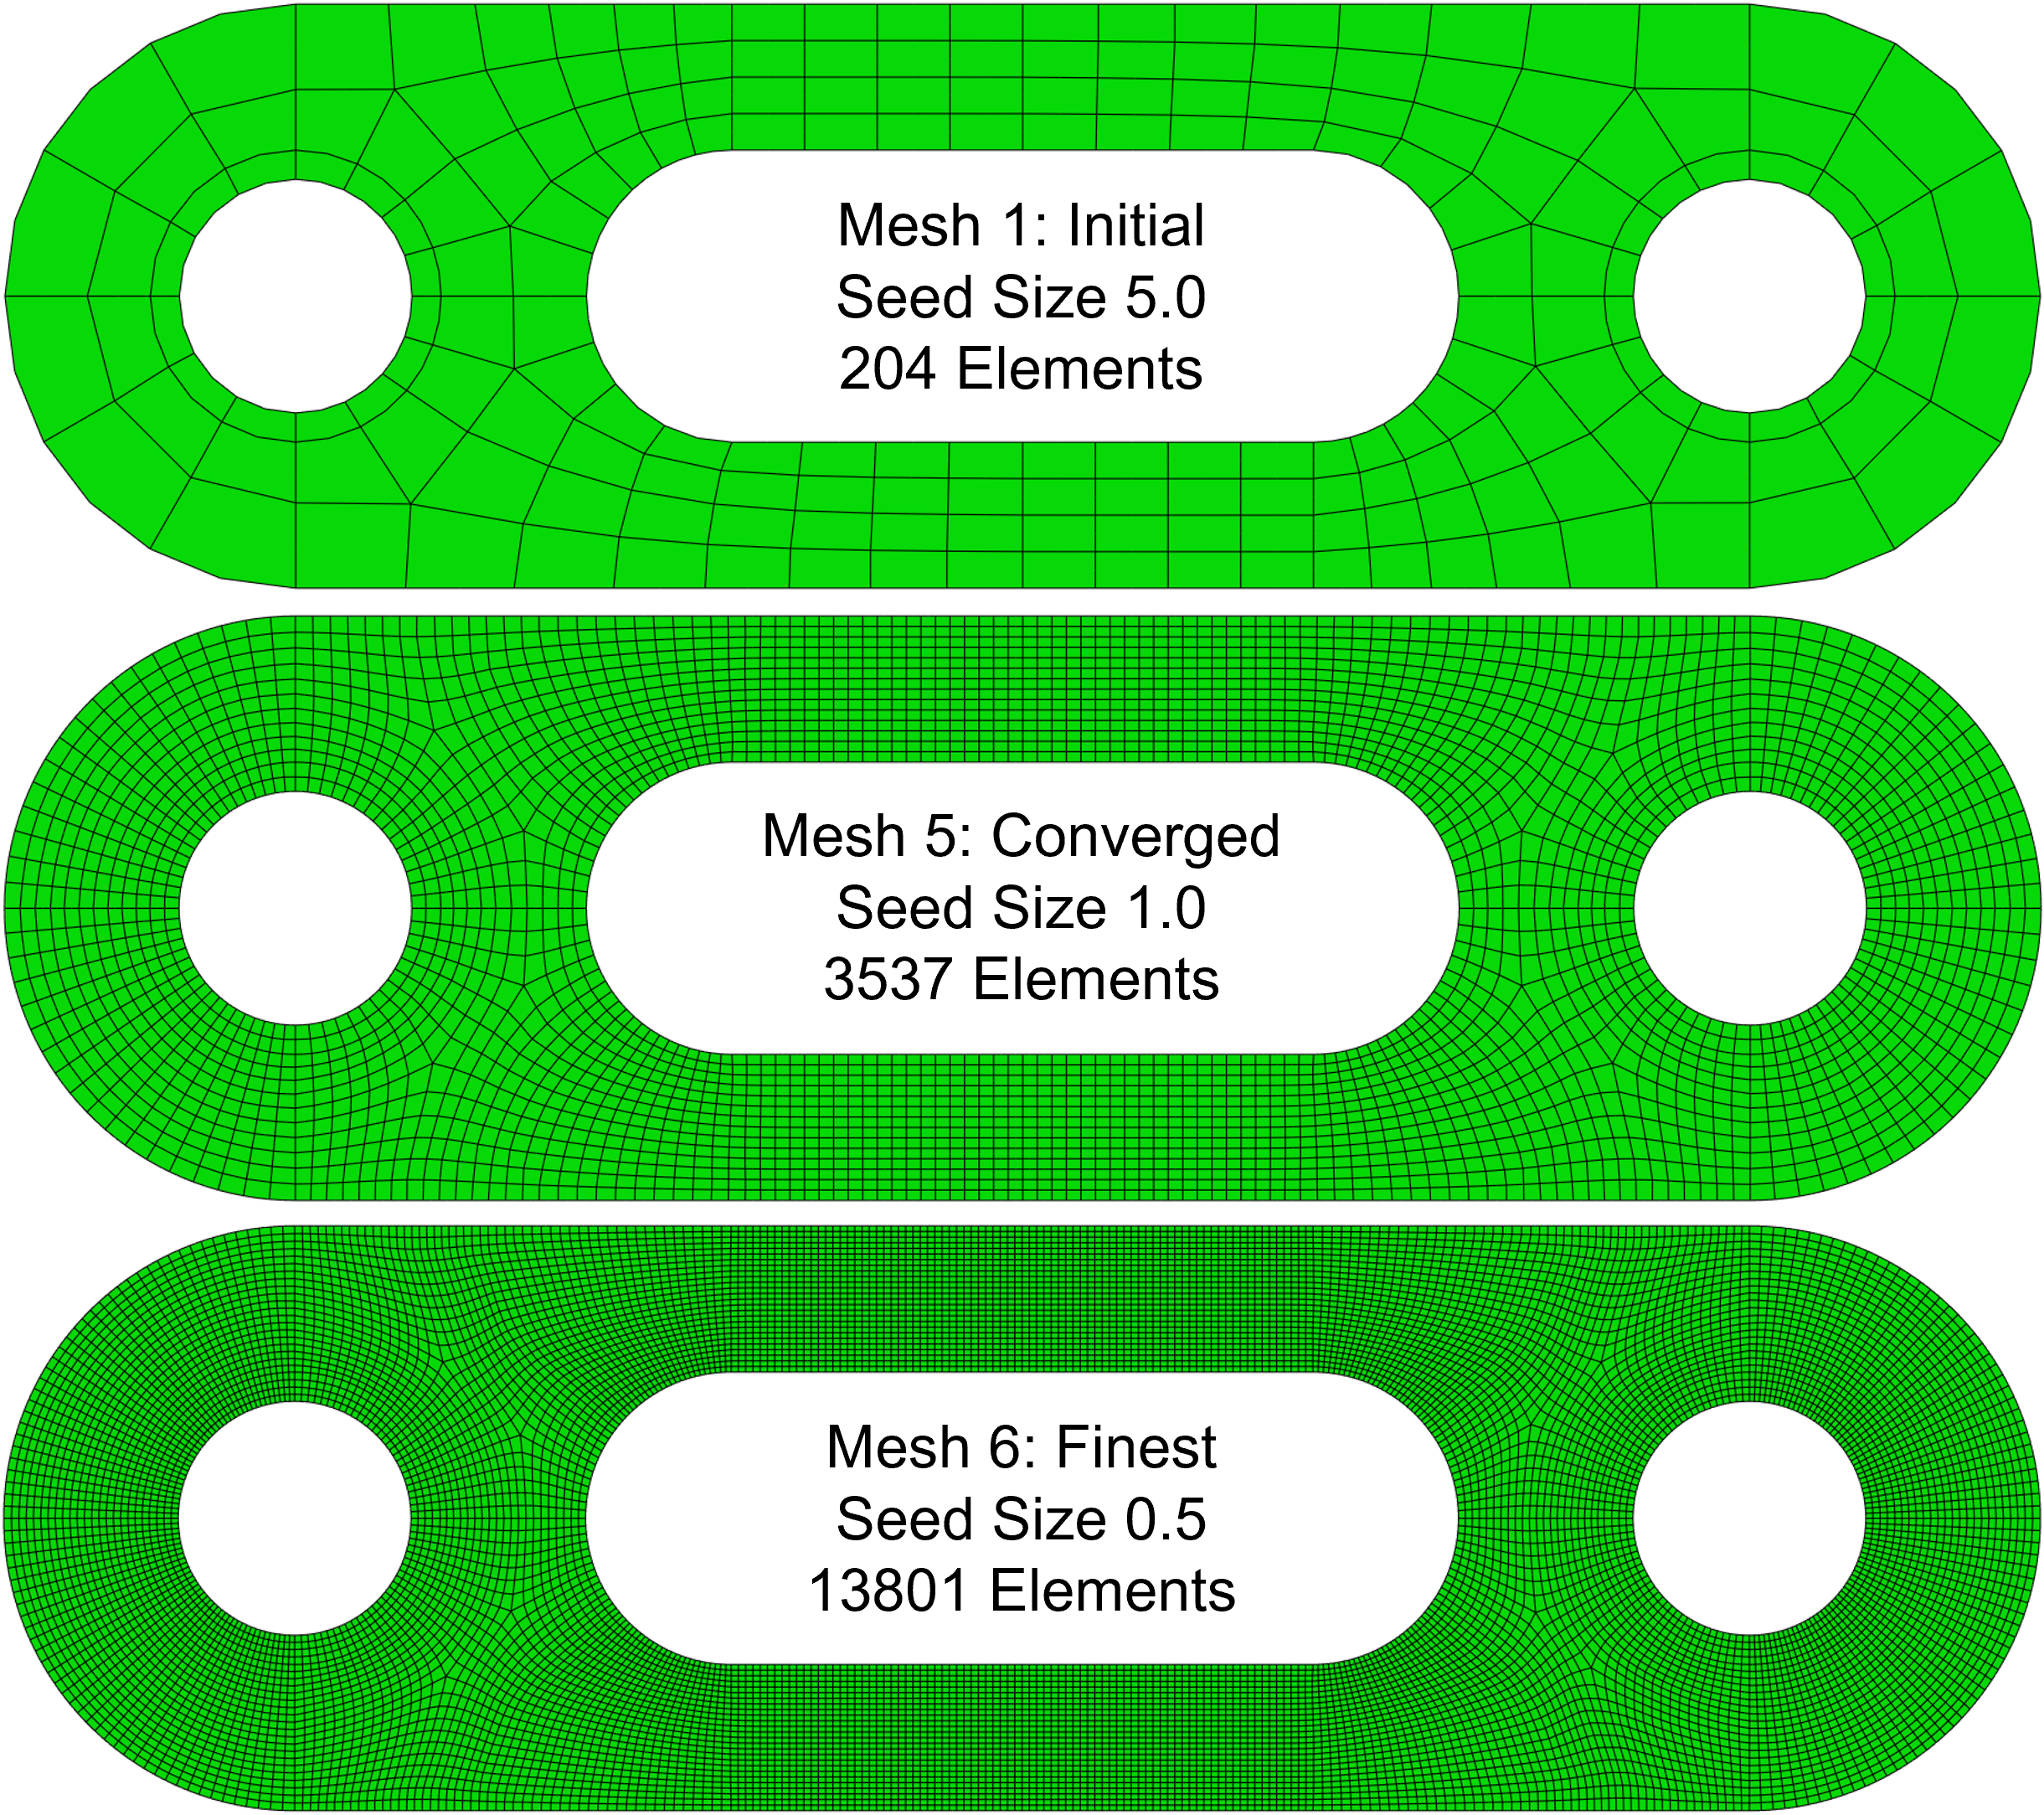
\includegraphics[scale=0.6]{../../images/meshes.png}
    \caption{Coarse, converged, and finest mesh.}
    \label{meshes}
\end{figure}

\begin{figure}[h!]
    \centering
    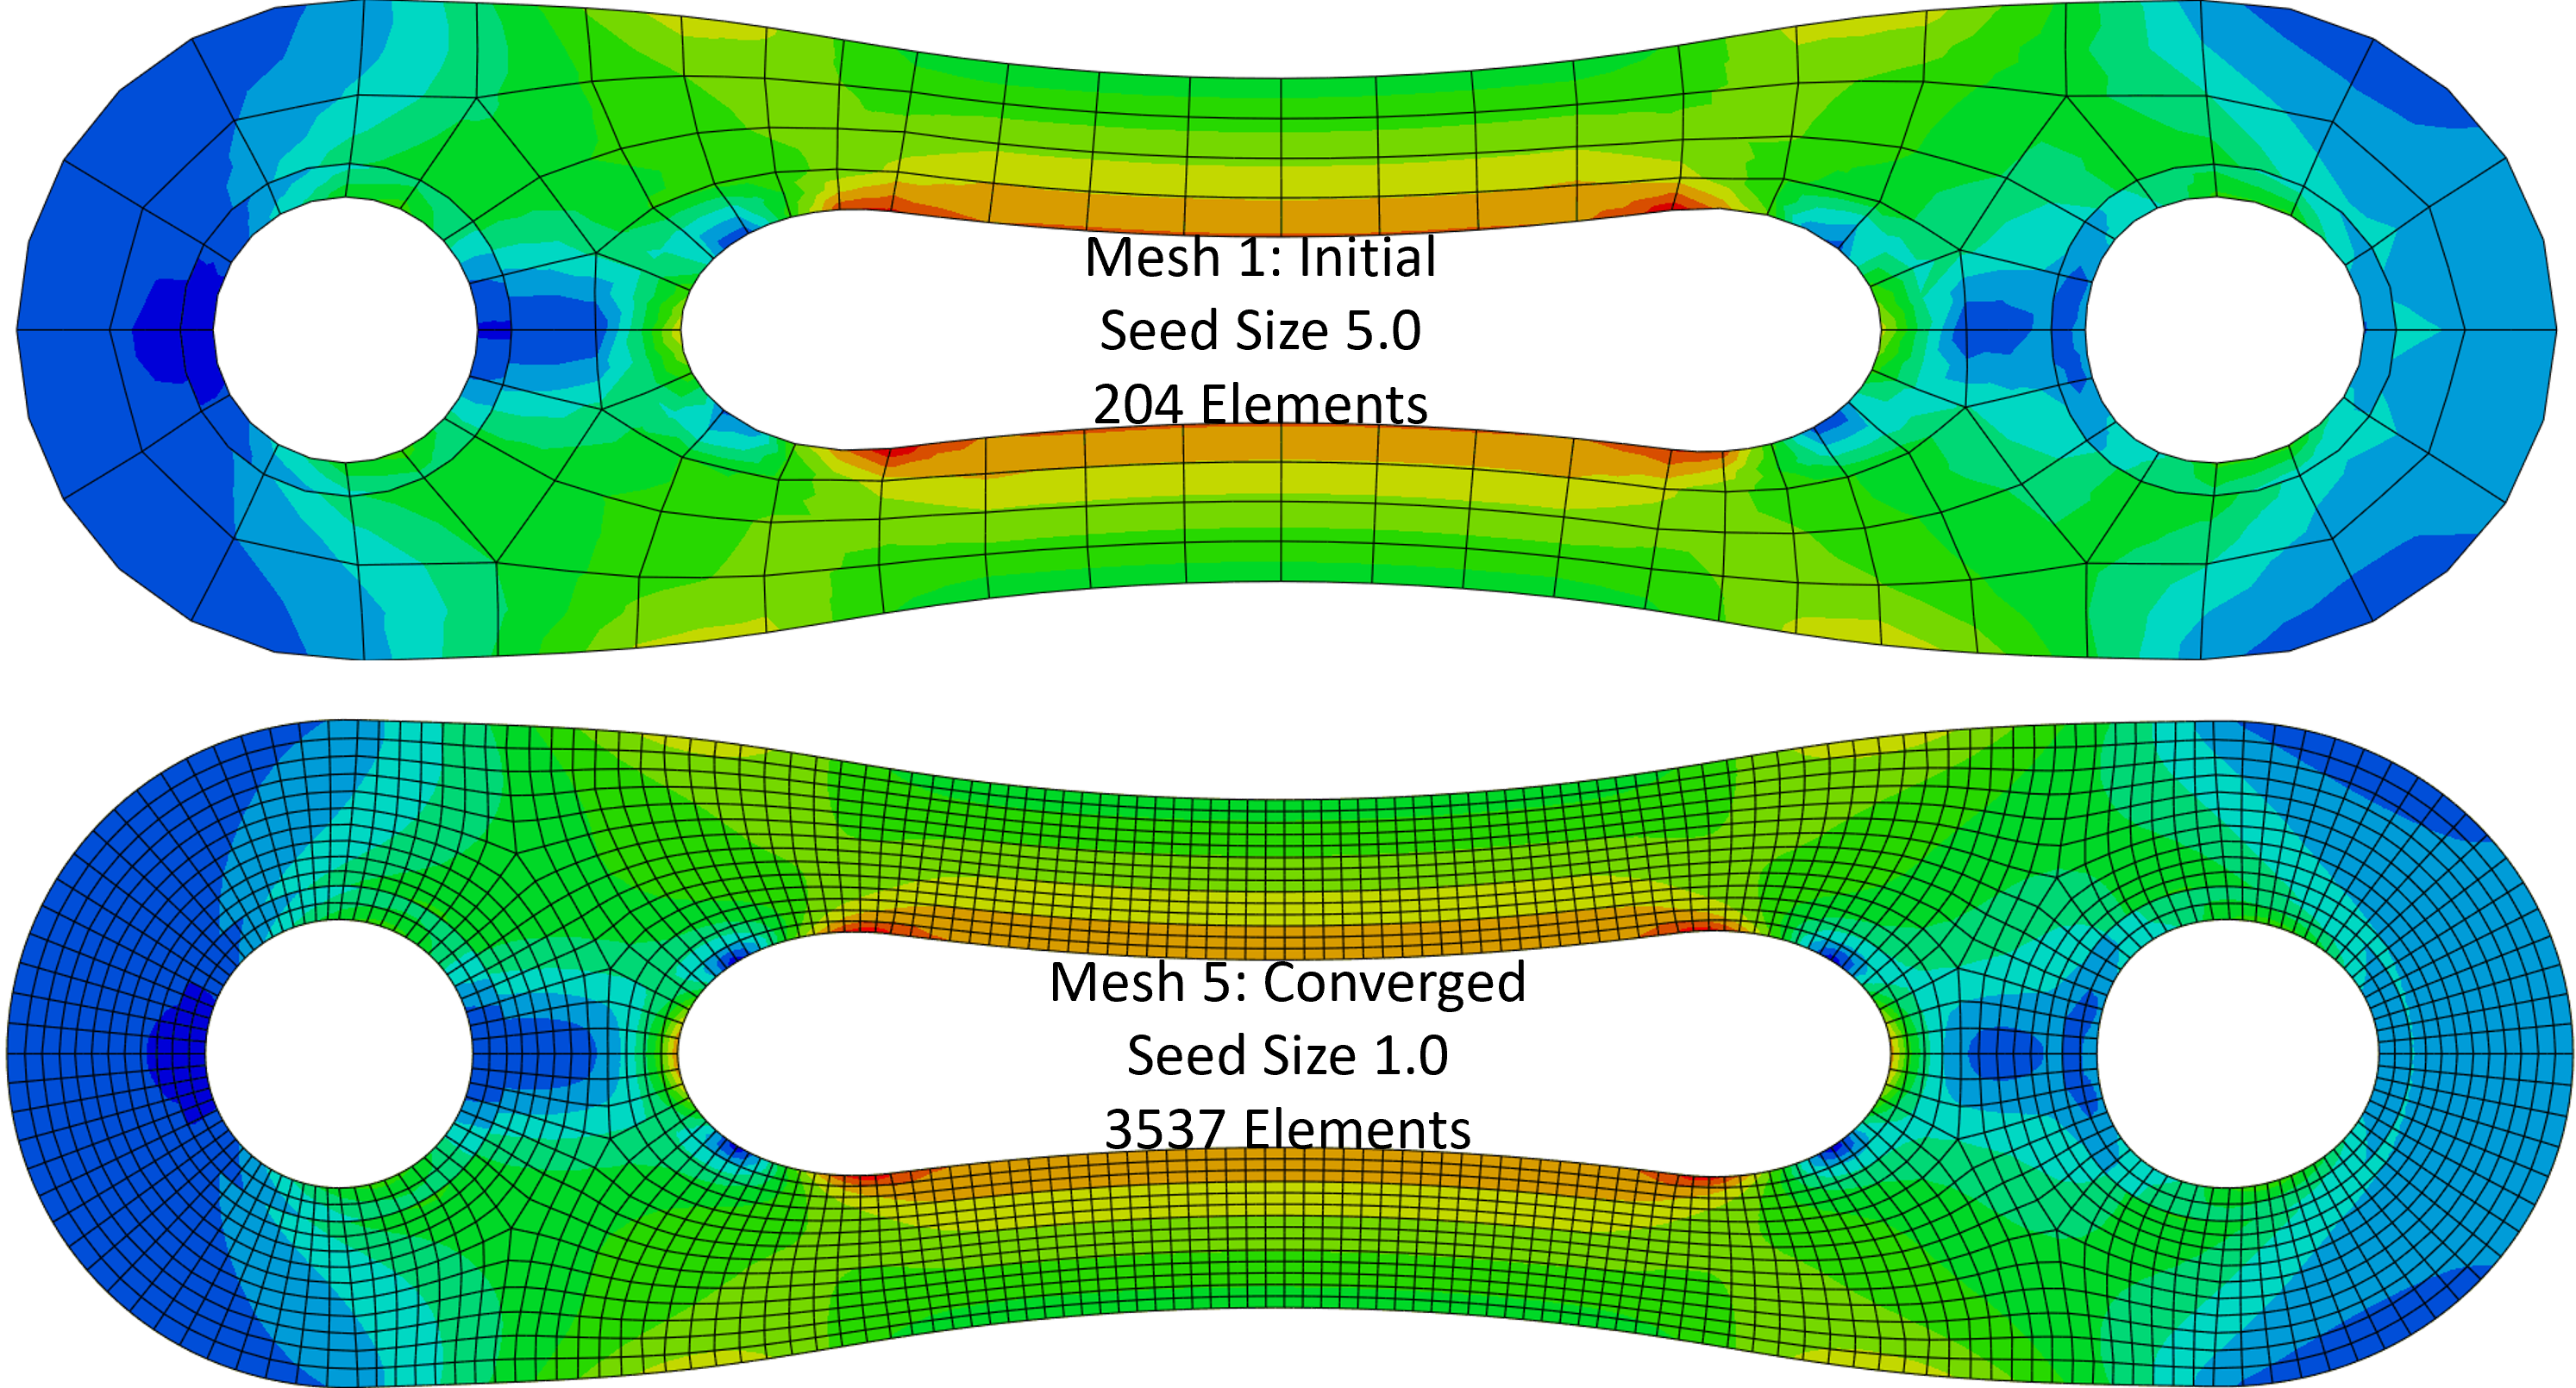
\includegraphics[scale=0.5]{../../images/coarse_vs_converged.png}
    \caption{Contour plots of Von Mises stress for initial and converged meshes}
    \label{coarse_vs_converged}
\end{figure}



\end{document}
